% $Id$
%==============================================================================
\section{Hello World Component}
\label{HelloWorldComponent}
%==============================================================================

As a quick tour through CCM Tools, we implement a simple Hello World 
component example (Fig.~\ref{fig:uml-helloworld}). 
Each development step and developer role will be described 
in more detail in one of the next sections, here we give a general overview.

\begin{figure}[htb]
    \begin{center}
        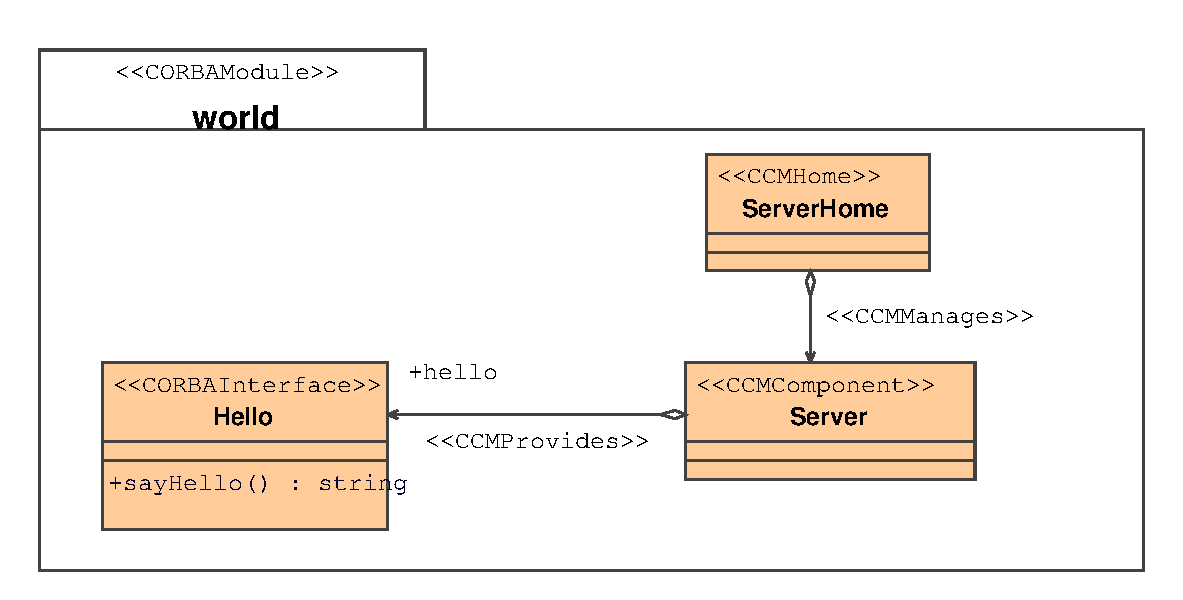
\includegraphics [width=12cm,angle=0] {uml/Hello.eps}
        \caption{A simple HelloWorld component example.}
        \label{fig:uml-helloworld}
    \end{center}
\end{figure}

\vspace{3mm}
\noindent
{\bf Step 1:} We define a component using the 
{\it Interface Definition Language} (IDL). 
This simple component only provides a single interface containing a single
method. Don't forget to define a home for this component type.
The following IDL definitions are stored in
a file called {\tt Hello.idl}:
\begin{small}
\begin{verbatim}
module world
{ 
    interface Hello 
    { 
        string sayHello(); 
    }; 

    component Server 
    { 
        provides Hello hello;
    }; 

    home ServerHome manages Server
    {
    };
};
\end{verbatim}
\end{small}


\noindent
{\bf Step 2:} Generate a uniform IDL3 structure from the single {\tt Hello.idl}
file:
\begin{small}
\begin{verbatim}
> ccmtools idl3 -o server/idl Hello.idl
\end{verbatim}
\end{small}

\noindent
This uniform IDL3 structure separates between interfaces (including 
parameter type and exception definitions) and components (including their
homes). Such a separation makes sense because an interface can be used by
many component definitions.
\begin{small}
\begin{verbatim}
    server/
     |-- idl
     |   |-- component
     |   |   `-- world
     |   |       |-- Server.idl
     |   |       `-- ServerHome.idl
     |   `-- interface
     |       `-- world
     |           `-- Hello.idl
\end{verbatim}
\end{small}


\noindent
{\bf Step 3:} Generate an empty component skeleton from the uniform IDL3 
structure:
\begin{small}
\begin{verbatim}
> ccmtools c++local -o server/interface \
                    -Iserver/idl/interface \
                    -Iserver/idl/component \
                    server/idl/interface/world/*.idl

> ccmtools c++local -a -o server/component/Server \ 
                    -Iserver/idl/interface \
                    -Iserver/idl/component \
                    server/idl/component/world/Server*.idl  
\end{verbatim}
\end{small}

\noindent
CCM Tools generate the following file structure which represents a local
component's implementation.
Code contained in the {\tt CCM\_*} directories establishes the component's
structure (= {\it component logic}), while code stored in the {\tt Server} 
directory represents the functional part of a component (= {\it business
logic}).

\begin{small}
\begin{verbatim}
   server
    |-- idl
    |-- component
    |   `-- Server
    |       |-- CCM_world_ccm_local_component_Server
    |       |-- CCM_world_ccm_local_component_Server_share
    |       |-- Makefile.py
    |       |-- ServerHome_impl.cc
    |       |-- ServerHome_impl.h
    |       |-- Server_hello_impl.cc
    |       |-- Server_hello_impl.h
    |       |-- Server_impl.cc
    |       |-- Server_impl.h
    |       `-- world_ccm_local_component_Server_ServerHome_entry.h
    `-- interface
        |-- CCM_world_ccm_local
        `-- CCM_world_ccm_local_adapter
\end{verbatim}
\end{small}

\noindent
{\bf Step 4:} Implement the component's business logic.
The component's business logic must be embedded in the generated
component logic. 
To implement the {\tt sayHello()} method of the {\tt Hello} interface,
we extend the generated {\tt Server\_hello\_impl.cc} file:
\begin{small}
\begin{verbatim}
std::string
hello_impl::sayHello()
    throw(::ccm::local::Components::CCMException)
{
    // TODO : IMPLEMENT ME HERE !
    return "Hello from Server component!";
}
\end{verbatim}
\end{small}

\noindent
Additionally, we create some {\tt Makefile.py} files which tell
{\tt confix} which package name, version and subdirectories
should be used.
\begin{small}
\begin{verbatim}
# server/Makefile.py
PACKAGE_NAME('HelloWorld')
PACKAGE_VERSION('1.0.0')
\end{verbatim}
\end{small}

\begin{small}
\begin{verbatim}
> touch server/interface/Makefile.py
> touch server/component/Makefile.py
> touch server/component/Server/Makefile.py
\end{verbatim}
\end{small}

\noindent
To compile and install this component, simply type: 
\begin{small}
\begin{verbatim}
> confix.py --packageroot=`pwd`/server --bootstrap --configure \
            --make --targets=install
\end{verbatim}
\end{small}


\noindent
{\bf Step 5:} Now we can implement a client that uses the Hello World
component. For this simple case, we implement the client as a {\tt \_check*}
file that will be automatically executed from a {\tt make check} command.

\begin{small}
\begin{verbatim}
   client/
   |-- Makefile.py
   `-- _check_client.cc
\end{verbatim}
\end{small}

\noindent
The following client code snippets are stored in the 
{\tt client/\_check\_client.cc} file:
\begin{small}
\begin{verbatim}
#include <WX/Utils/debug.h>
#include <WX/Utils/smartptr.h>

#include <ccm/local/Components/CCM.h>
#include <ccm/local/HomeFinder.h>

#include <world/ccm/local/component/Server/Server_gen.h>
#include <world/ccm/local/component/Server/ServerHome_gen.h>

using namespace std;
using namespace WX::Utils;
using namespace world::ccm::local;

int main(int argc, char *argv[])
{
    SmartPtr<component::Server::Server> server;
    SmartPtr<Hello> hello;
    ccm::local::Components::HomeFinder* homeFinder =
      ccm::local::HomeFinder::Instance();
    int error;

    try {

      // Deploy component type
      error = deploy_world_ccm_local_component_Server_ServerHome("ServerHome");
      if(error) {
        cerr << "BOOTSTRAP ERROR: Can't deploy component homes!" << endl;
        return(error);
      }
      
      // Instantiate component
      SmartPtr<component::Server::ServerHome> 
          home(dynamic_cast<component::Server::ServerHome*>
          (homeFinder->find_home_by_name("ServerHome").ptr()));
      server = home->create();   
      hello = server->provide_hello();
      server->configuration_complete();
    
      // Use component instance
      string s = hello->sayHello();
      cout << "sayHello(): " << s << endl;

      // Destroy component instance
      server->remove();

      // Undeploy component type
      error += undeploy_world_ccm_local_component_Server_ServerHome("ServerHome");
      if(error) {
        cerr << "ERROR: Can't undeploy component homes!" << endl;
        return(error);
      }
    } 
    catch ( ccm::local::Components::HomeNotFound ) {
        cout << "ERROR: can't find a home!" << endl;
        error = -1;
    } 
    catch ( ccm::local::Components::NotImplemented& e ) {
        cout << "ERROR: function not implemented: " 
	     << e.what (  ) << endl;
        error = -1;
    }  
    catch ( ccm::local::Components::InvalidName& e ) {
        cout << "ERROR: invalid name during connection: " 
             << e.what (  ) << endl;
        error = -1;
    }

    // Clean up singleton
    ccm::local::HomeFinder::destroy();
}
\end{verbatim}
\end{small}


\noindent
Again, we write a {\tt client/Makefile.py} that tells {\tt confix} the
name and version of the client package.
\begin{small}
\begin{verbatim}
PACKAGE_NAME('HelloClient')
PACKAGE_VERSION('1.0.0')
\end{verbatim}
\end{small}

\noindent
To compile and run the component's client, type the following {\tt confix}
line: 
\begin{small}
\begin{verbatim}
> confix.py --packageroot=`pwd`/client --bootstrap --configure \
            --make --targets=check
\end{verbatim}
\end{small}

\noindent
After all, we are happy to see the following output at the end of the client's
build process:

\begin{small}
\begin{verbatim}
sayHello(): Hello from Server component!
PASS: hello-client__check_client
==================
All 1 tests passed
==================
\end{verbatim}
\end{small}

\noindent
Of course, to implement a component for a simple 'Hello from Server component!'
message is somewhat academical, but this example shows how simple a component
development cycle can be. 
The intent of this section was to define the main activities in component 
development, which are:
\begin{itemize}
\item Define a component's structure (using IDL or UML).
\item Generate an empty component skeleton (called component logic).
\item Implement a component's business logic. 
\item Implement a component's client.
\end{itemize}

\noindent
In the following sections, we will explore each of these steps in more
detail. However, keep this big picture in mind. 

